% Compile with: pdflatex presentation.tex (twice)
% Requires the `metropolis` theme (TeX Live: package `beamertheme-metropolis`).
% If unavailable, change \usetheme{metropolis} to \usetheme{default} below.

\documentclass[10pt,aspectratio=169]{beamer}

\usetheme{metropolis}
\metroset{progressbar=frametitle, sectionpage=progressbar, numbering=fraction}

\usepackage{booktabs}
\usepackage{graphicx}
\usepackage{amsmath}
\usepackage{xcolor}

\definecolor{accent}{HTML}{2980b9}
\definecolor{good}{HTML}{27ae60}
\definecolor{bad}{HTML}{c0392b}
\setbeamercolor{progress bar}{fg=accent}
\setbeamercolor{title separator}{fg=accent}

\setbeamerfont{title}{size=\Large, series=\bfseries}
\setbeamerfont{frametitle}{size=\normalsize, series=\bfseries}
\setbeamerfont{caption}{size=\scriptsize}

\newcommand{\tk}[1]{{\scriptsize \textcolor{accent}{$\blacktriangleright$}\ #1}}

\title{Learning to Prune --- Part II}
\subtitle{What sets prunability, why RL is vestigial, and a cautionary tale about ``cleaner'' objectives}
\author{Keshava Pampatti}
\date{\today}

\graphicspath{{./}}

\begin{document}

\maketitle

% ============================================================
\begin{frame}{Where we were}
  \begin{itemize}
    \item A small \textbf{weight-conditioned hypernetwork} (BiLSTM) reads the trained weights and emits a per-neuron keep/drop gate.
    \item Last time: it prunes well, scales with width, and an RL/MDP variant pushes sparsity higher.
  \end{itemize}
  \vspace{0.8em}
  \begin{block}{Since then --- this talk}
    The project became a \emph{science} program: \emph{what} determines prunability, \emph{whether} the sequential framing helps, \emph{what} transfers --- and a hard-won lesson about replacing a soft penalty with a hard budget.
  \end{block}
\end{frame}

% ============================================================
\section{Recap: the hypernetwork works}
% ============================================================

\begin{frame}{Weights alone encode redundancy --- and it's near-deterministic}
  \begin{columns}[T,onlytextwidth]
    \column{0.52\textwidth}
      \textbf{F1.} Reading \emph{only} the weight matrices (no data, no gradients), the BiLSTM prunes \textbf{60--79\%} of hidden neurons at $<$0.1--3.7pp accuracy drop.
      \vspace{0.6em}

      \textbf{F2.} Re-run with fresh pruner seeds $\Rightarrow$ \emph{same mask}. Dead/alive activation ratio $\sigma = \mathbf{0.007}$.
      \vspace{0.4em}

      \tk{The redundancy readout is a \emph{fixed property of the network}, not an artifact of pruner init.}
    \column{0.48\textwidth}
      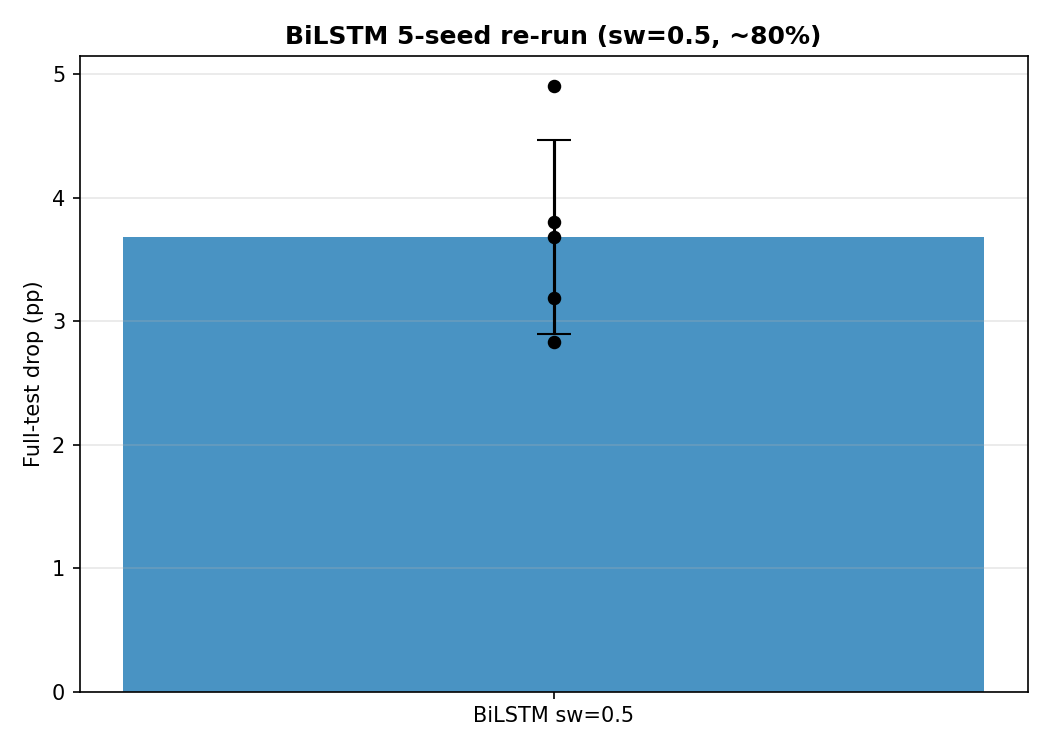
\includegraphics[width=\linewidth]{f2_5seed.png}
  \end{columns}
\end{frame}

\begin{frame}{Learned pruning strictly dominates heuristics}
  \begin{columns}[T,onlytextwidth]
    \column{0.5\textwidth}
      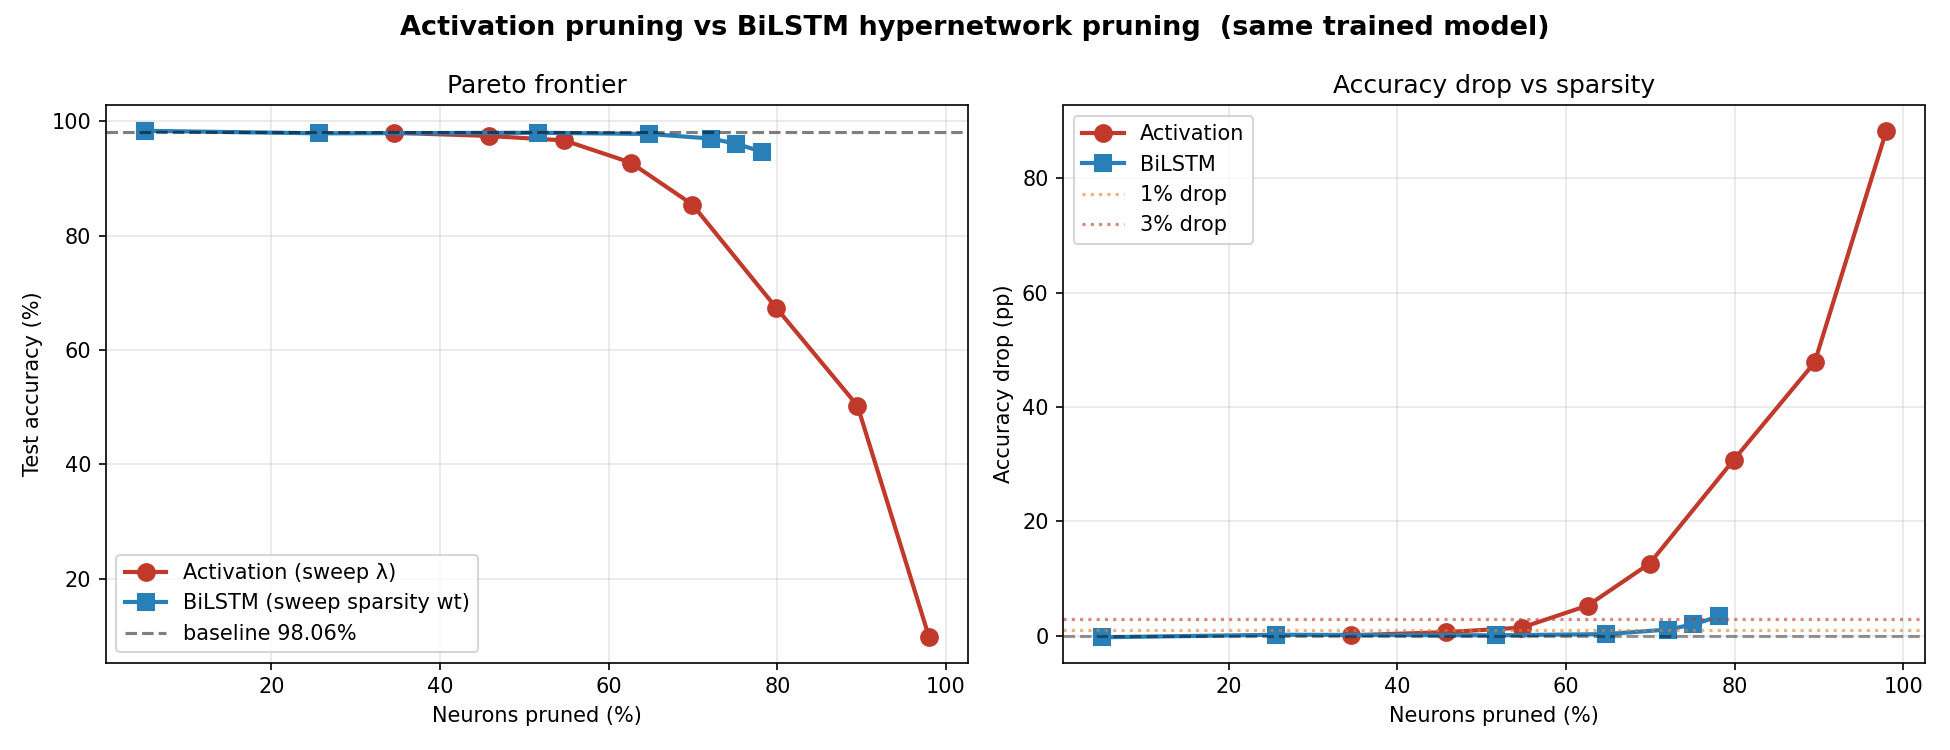
\includegraphics[width=\linewidth]{f3_act_vs_bilstm.png}
    \column{0.5\textwidth}
      \textbf{F3.} At every accuracy budget the BiLSTM prunes more than activation/magnitude.
      \vspace{0.6em}
      \begin{center}\small
      \begin{tabular}{@{}lrr@{}}
        \toprule
        Drop $\leq$ & Activation & BiLSTM \\
        \midrule
        0.5\% & 34.5\% & \textbf{64.7\%} \\
        1.0\% & 45.8\% & \textbf{72.1\%} \\
        3.0\% & 54.7\% & \textbf{75.1\%} \\
        \bottomrule
      \end{tabular}
      \end{center}
      \vspace{0.5em}
      \tk{Activation falls off a cliff past 50\%; BiLSTM holds $\leq$2\% to 75\%.}
  \end{columns}
\end{frame}

% ============================================================
\section{What determines prunability?}
% ============================================================

\begin{frame}{Prunability scales with WIDTH, not size}
  \begin{columns}[T,onlytextwidth]
    \column{0.52\textwidth}
      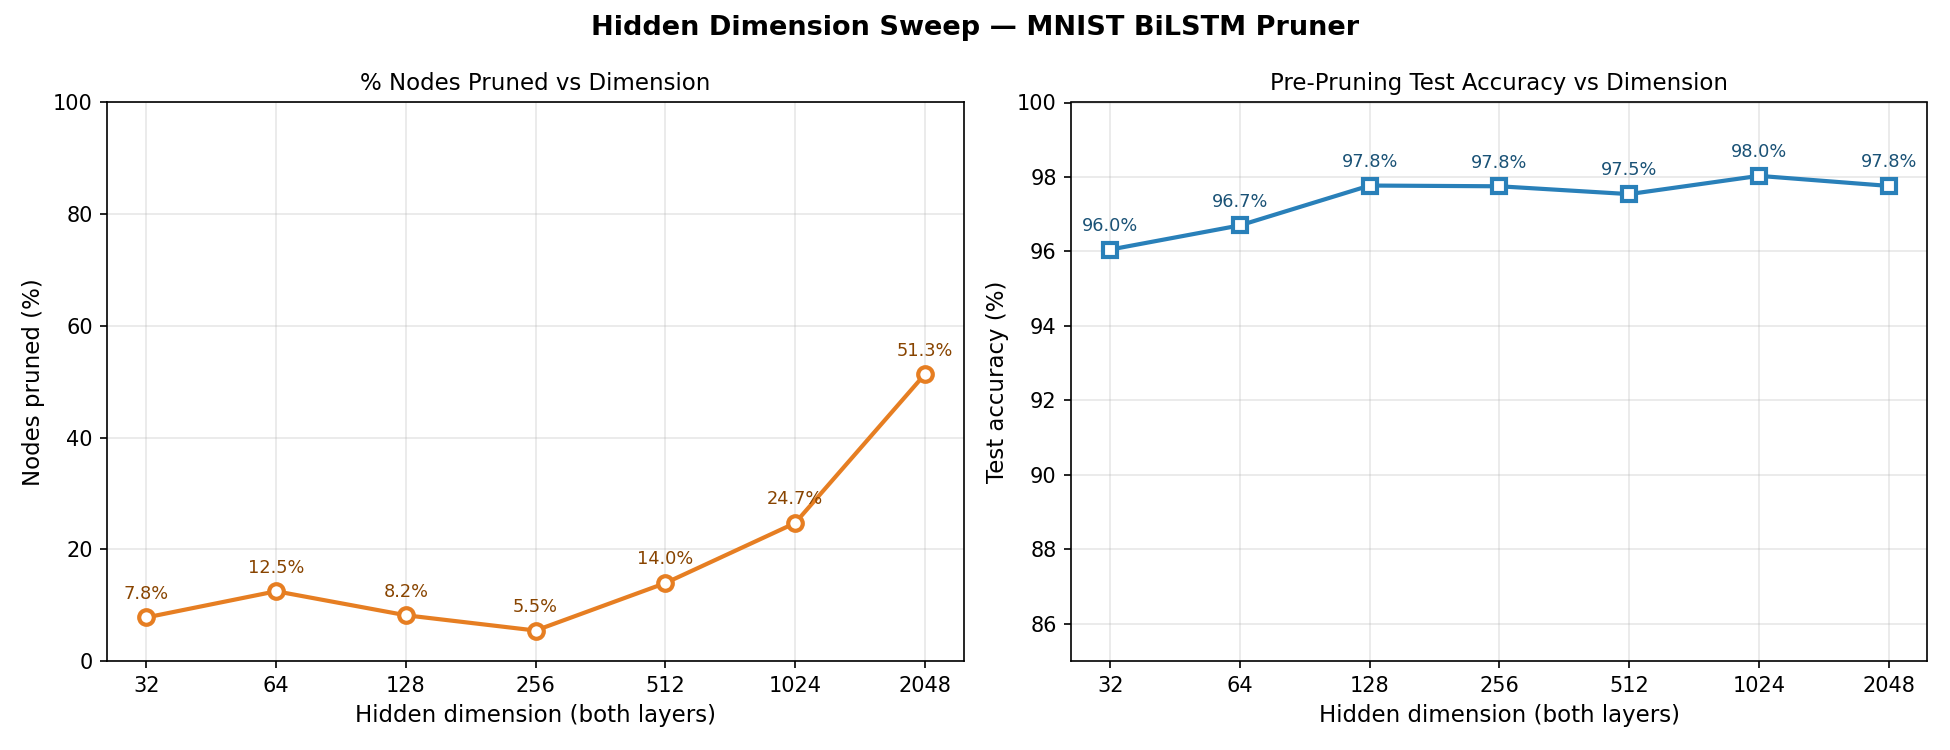
\includegraphics[width=\linewidth]{f4_dim_sweep.png}
    \column{0.48\textwidth}
      \textbf{F4.} Same task, vary hidden width: prunability is \emph{monotonic} in width.
      \begin{itemize}
        \item dim 32 $\to$ \textbf{8\%} removable.
        \item dim 2048 $\to$ \textbf{51\%}.
      \end{itemize}
      \vspace{0.4em}
      At a \emph{fixed} 2048-neuron budget, trading width for depth still loses prunability (wide 93\% $>$ medium 79\% $>$ deep 58\%).
      \vspace{0.5em}

      \tk{\textbf{Q4 answered:} prunability is set by how redundancy is \emph{distributed} (width), not by parameter count.}
  \end{columns}
\end{frame}

% ============================================================
\section{Shape and the conserved quantity}
% ============================================================

\begin{frame}{Iso-accuracy: width is cheap, depth is load-bearing}
  \begin{columns}[T,onlytextwidth]
    \column{0.5\textwidth}
      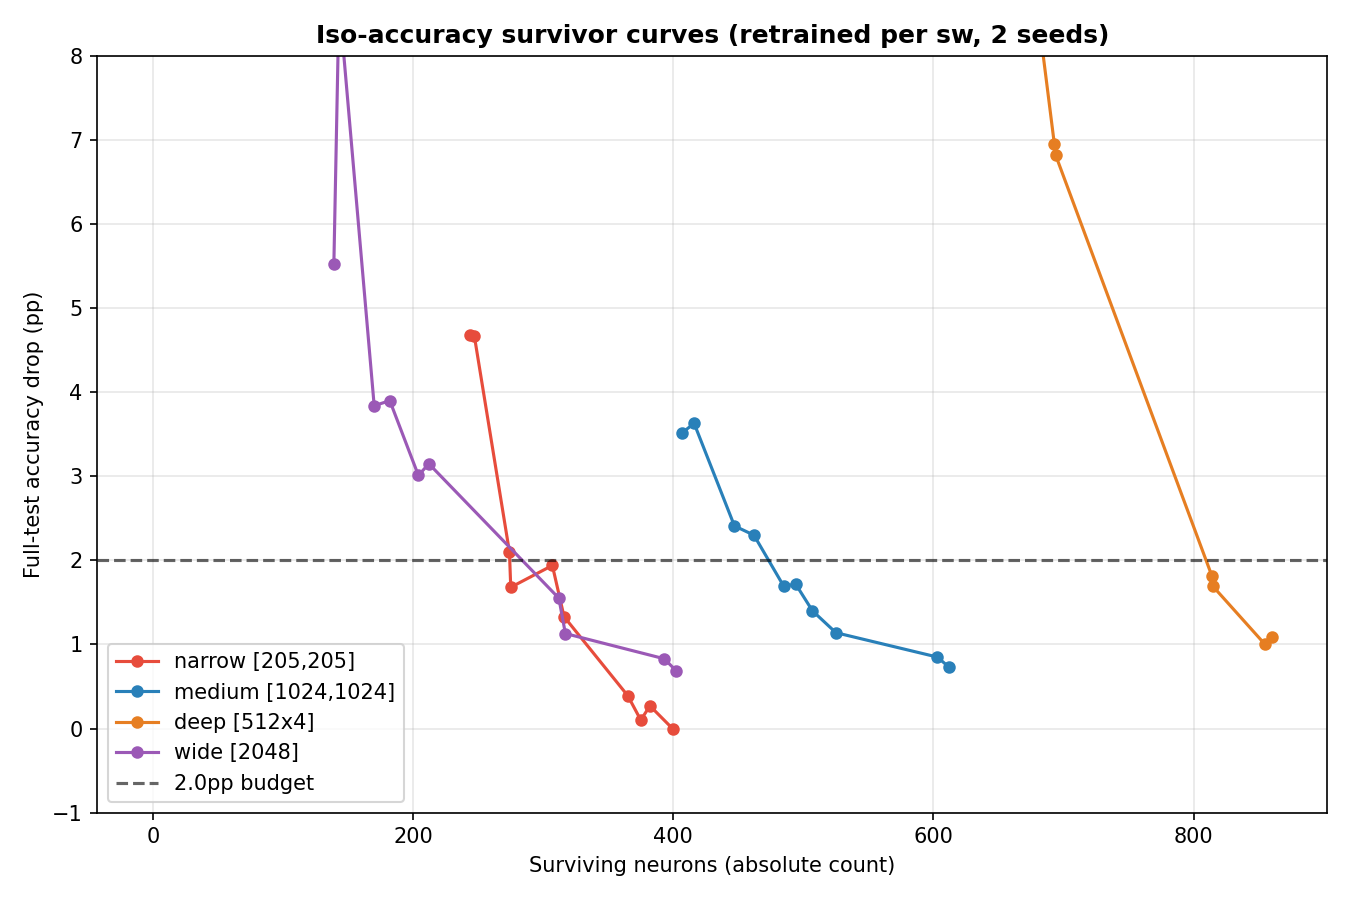
\includegraphics[width=\linewidth]{f10_curves.png}
    \column{0.5\textwidth}
      \textbf{F10.} Prune each shape to a fixed 2pp drop (pruner retrained per sparsity).
      \begin{center}\scriptsize
      \begin{tabular}{@{}lrrr@{}}
        \toprule
        Shape & Layers & Surv.\ @2pp & \% pruned \\
        \midrule
        wide [2048]      & 1 & 314 & \textbf{84.6} \\
        medium [1024$^2$]& 2 & 490 & 76.1 \\
        deep [512$\times$4] & 4 & 814 & 60.2 \\
        narrow [205$^2$] & 2 & 296 & 27.9 \\
        \bottomrule
      \end{tabular}
      \end{center}
      \vspace{0.3em}
      \tk{Prunability $\uparrow$ with width; but the \emph{minimal subnetwork grows with depth} (314$\to$490$\to$814 for 1/2/4 layers). \textbf{Q9: no universal neuron floor.}}
  \end{columns}
\end{frame}

\begin{frame}{Neurons are packaging --- \emph{weights} are conserved}
  \begin{columns}[T,onlytextwidth]
    \column{0.5\textwidth}
      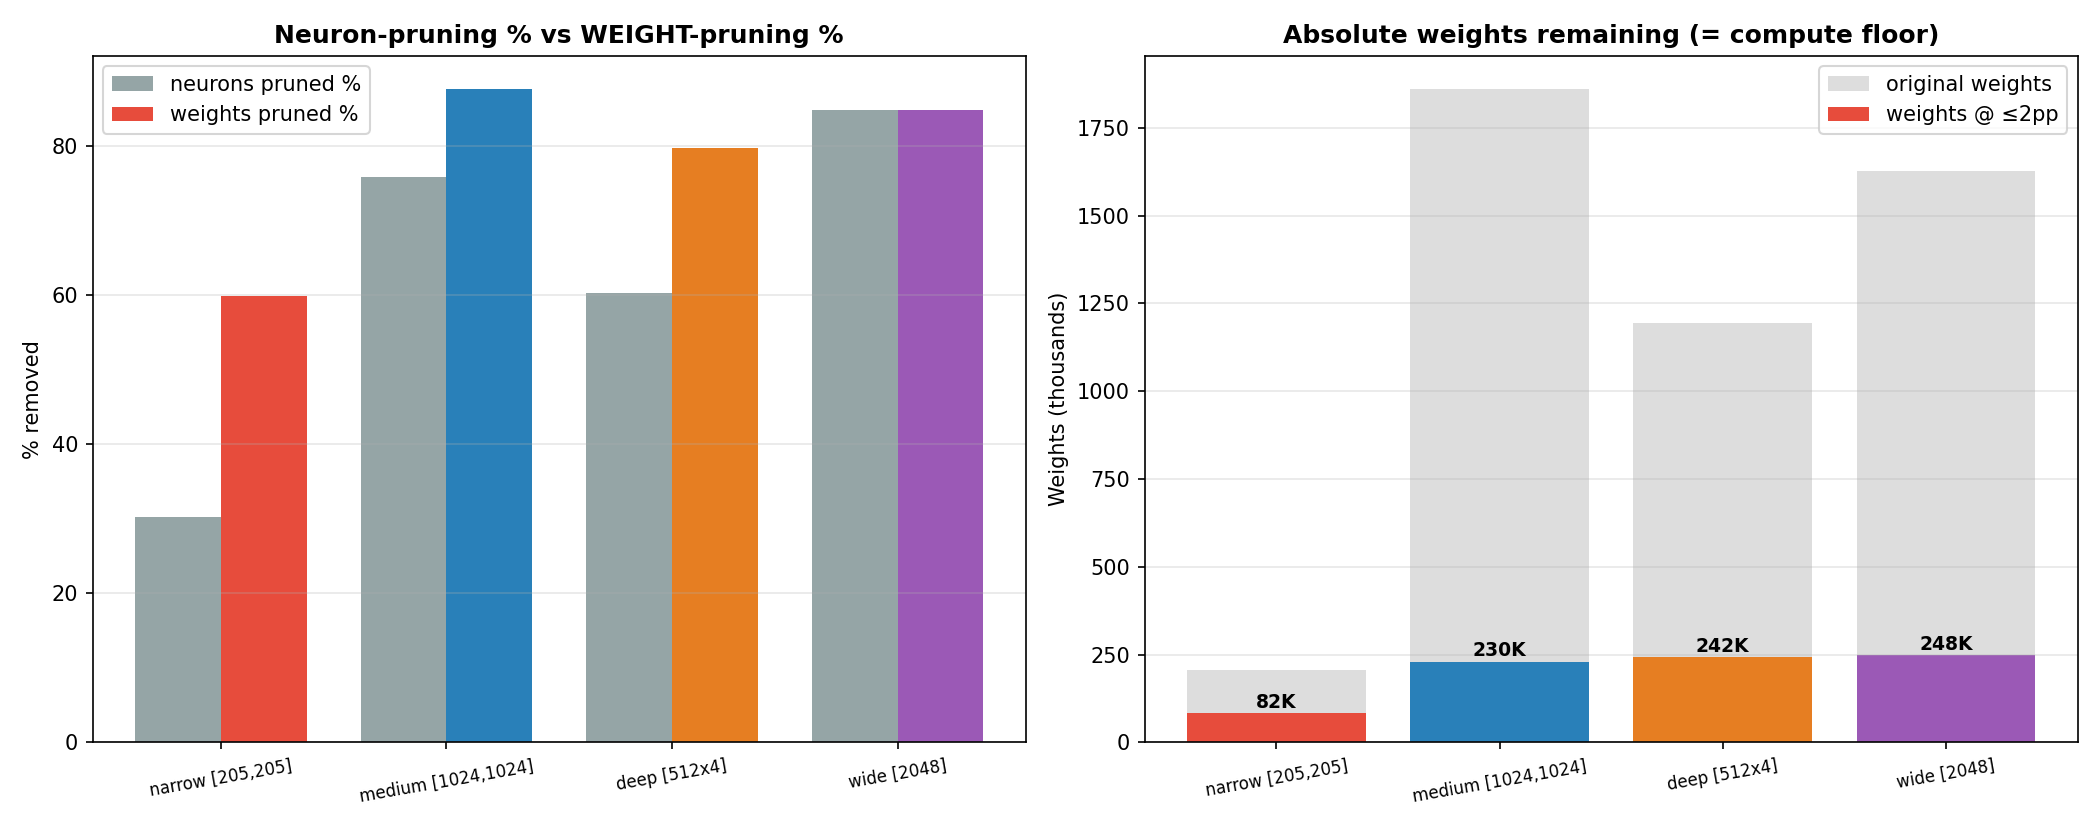
\includegraphics[width=\linewidth]{f11_weights.png}
    \column{0.5\textwidth}
      \textbf{F11.} Dropping a hidden neuron removes its in-row \emph{and} out-column. Hidden$\to$hidden matrices prune two-sided:
      \[ \text{weights kept} \;\propto\; (1-f)^2 \quad\text{(quadratic)} \]
      \begin{center}\scriptsize
      \begin{tabular}{@{}lrr@{}}
        \toprule
        Shape & Neurons -\% & \textbf{Weights @2pp} \\
        \midrule
        medium & 75.9 & \textbf{230K} \\
        deep   & 60.3 & \textbf{242K} \\
        wide   & 84.8 & \textbf{248K} \\
        \bottomrule
      \end{tabular}
      \end{center}
      \vspace{0.3em}
      \tk{Three different 2048-nets all land at $\sim$\textbf{240K weights} --- an architecture-invariant compute floor for MNIST@2pp.}
  \end{columns}
\end{frame}

\begin{frame}{Pruning-from-big $\neq$ training-small}
  \begin{columns}[T,onlytextwidth]
    \column{0.55\textwidth}
      \begin{itemize}
        \item Pruning any big net bottoms out at $\sim$\textbf{240K} weights @2pp.
        \item A network \emph{trained} small (narrow [205,205]) reaches the same accuracy at \textbf{82K} weights.
      \end{itemize}
      \vspace{0.6em}
      \[ \underbrace{240\text{K}}_{\text{prune-from-big}} \;\approx\; 3\times \underbrace{82\text{K}}_{\text{train-small}} \]
      \vspace{0.2em}
      \tk{Pruning leaves $\sim$3$\times$ irreducible redundancy --- it does not find the true minimal solution (echoes Liu et al.\ 2019).}
    \column{0.45\textwidth}
      \begin{block}{Reading}
        ``Capacity'' is not a scalar. Width = cheap parallel redundancy; depth = required serial capacity; the conserved quantity is \emph{compute} ($\approx$240K MACs), not neurons.
      \end{block}
  \end{columns}
\end{frame}

% ============================================================
\section{Why RL doesn't help here}
% ============================================================

\begin{frame}{Pruning a frozen net is functionally non-sequential}
  The base weights are \textbf{frozen} --- there is \emph{no weight update between prune steps}.
  \vspace{0.4em}
  \begin{itemize}
    \item The only thing that changes step-to-step is \emph{which neurons remain} (the mask).
    \item So final accuracy is a \textbf{set function} of the kept subset --- independent of the \emph{order} of removals: ``remove A then B'' $=$ ``remove B then A''.
    \item There is no temporal structure for a policy to exploit.
  \end{itemize}
  \vspace{0.5em}
  \begin{block}{Consequence}
    Pruning here is \emph{static subset selection} wearing an MDP costume. A method that optimises the mask \textbf{directly} --- the differentiable hypernetwork --- is the \textbf{theoretical ceiling} for any RL policy on a frozen net.
  \end{block}
  \vspace{0.3em}
  \tk{\textbf{Q7 / the escape:} the MDP turns genuinely sequential only if weights \emph{co-adapt} --- an update \emph{between} steps (prune \emph{during} training).}
\end{frame}

% ============================================================
\section{What transfers}
% ============================================================

\begin{frame}{The method transfers; the weights don't}
  \begin{columns}[T,onlytextwidth]
    \column{0.5\textwidth}
      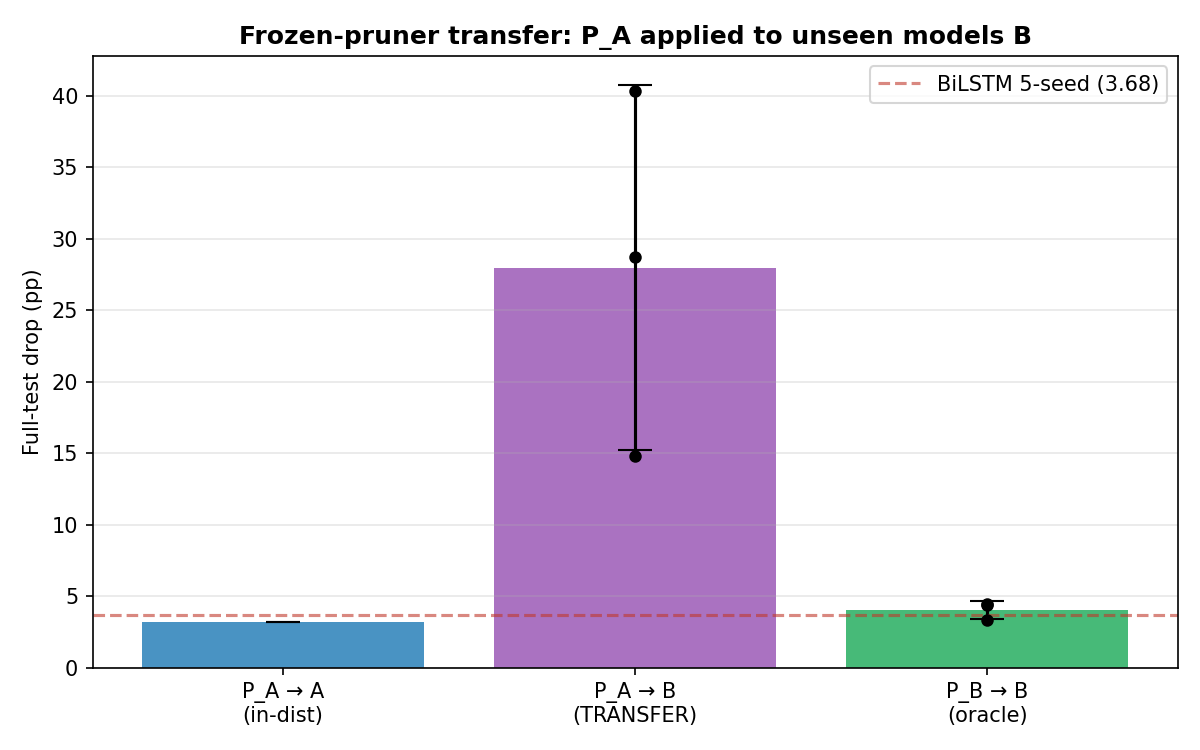
\includegraphics[width=\linewidth]{f7_transfer.png}
    \column{0.5\textwidth}
      \textbf{F7.} Take pruner trained on net A, apply to a fresh net B (same architecture):
      \begin{center}\small
      \begin{tabular}{@{}lr@{}}
        \toprule
        Condition & Drop (pp) \\
        \midrule
        $P_A \to A$ (in-dist.) & 3.19 \\
        $P_A \to B$ (transfer) & \textbf{27.96 $\pm$ 12.8} \\
        $P_B \to B$ (oracle) & 4.04 $\pm$ 0.6 \\
        \bottomrule
      \end{tabular}
      \end{center}
      \vspace{0.4em}
      \tk{Redundancy is idiosyncratic per network (a permutation frame). The BiLSTM is a reliable \emph{procedure}, not a portable \emph{answer}. \textbf{Q6:} a meta-trained detector is still open.}
  \end{columns}
\end{frame}

% ============================================================
\section{A cautionary tale: top-K}
% ============================================================

\begin{frame}{Can we drop the per-model $\lambda$ sweep?}
  \begin{columns}[T,onlytextwidth]
    \column{0.55\textwidth}
      Current pruner uses a soft penalty; the sparsity \emph{emerges} and $\lambda$ must be swept per model (8$\times$ across shapes):
      \[ \mathcal{L} = (\text{CE}_{\text{pr}} - \text{CE}_{\text{orig}}) + \lambda\,\overline{\text{gate}} \]
      \textbf{Idea:} hard \textbf{global top-K} --- set the budget $K$ directly, learn only \emph{which} $K$ to keep. No $\lambda$, no collapse-prevention hacks.
      \vspace{0.4em}

      \tk{Cleaner and sweep-free \emph{in principle}. In practice it opened a trap-door.}
    \column{0.45\textwidth}
      \begin{block}{What we expected}
        Same accuracy floor as $\lambda$, minus the per-model tuning and the stabilisation hacks.
      \end{block}
      \begin{block}{\textcolor{bad}{What happened}}
        A deterministic collapse to one class (88.3pp), reproducible bit-for-bit across configs.
      \end{block}
  \end{columns}
\end{frame}

\begin{frame}{Pathology \#1 --- global top-K starves a layer to death}
  \begin{columns}[T,onlytextwidth]
    \column{0.52\textwidth}
      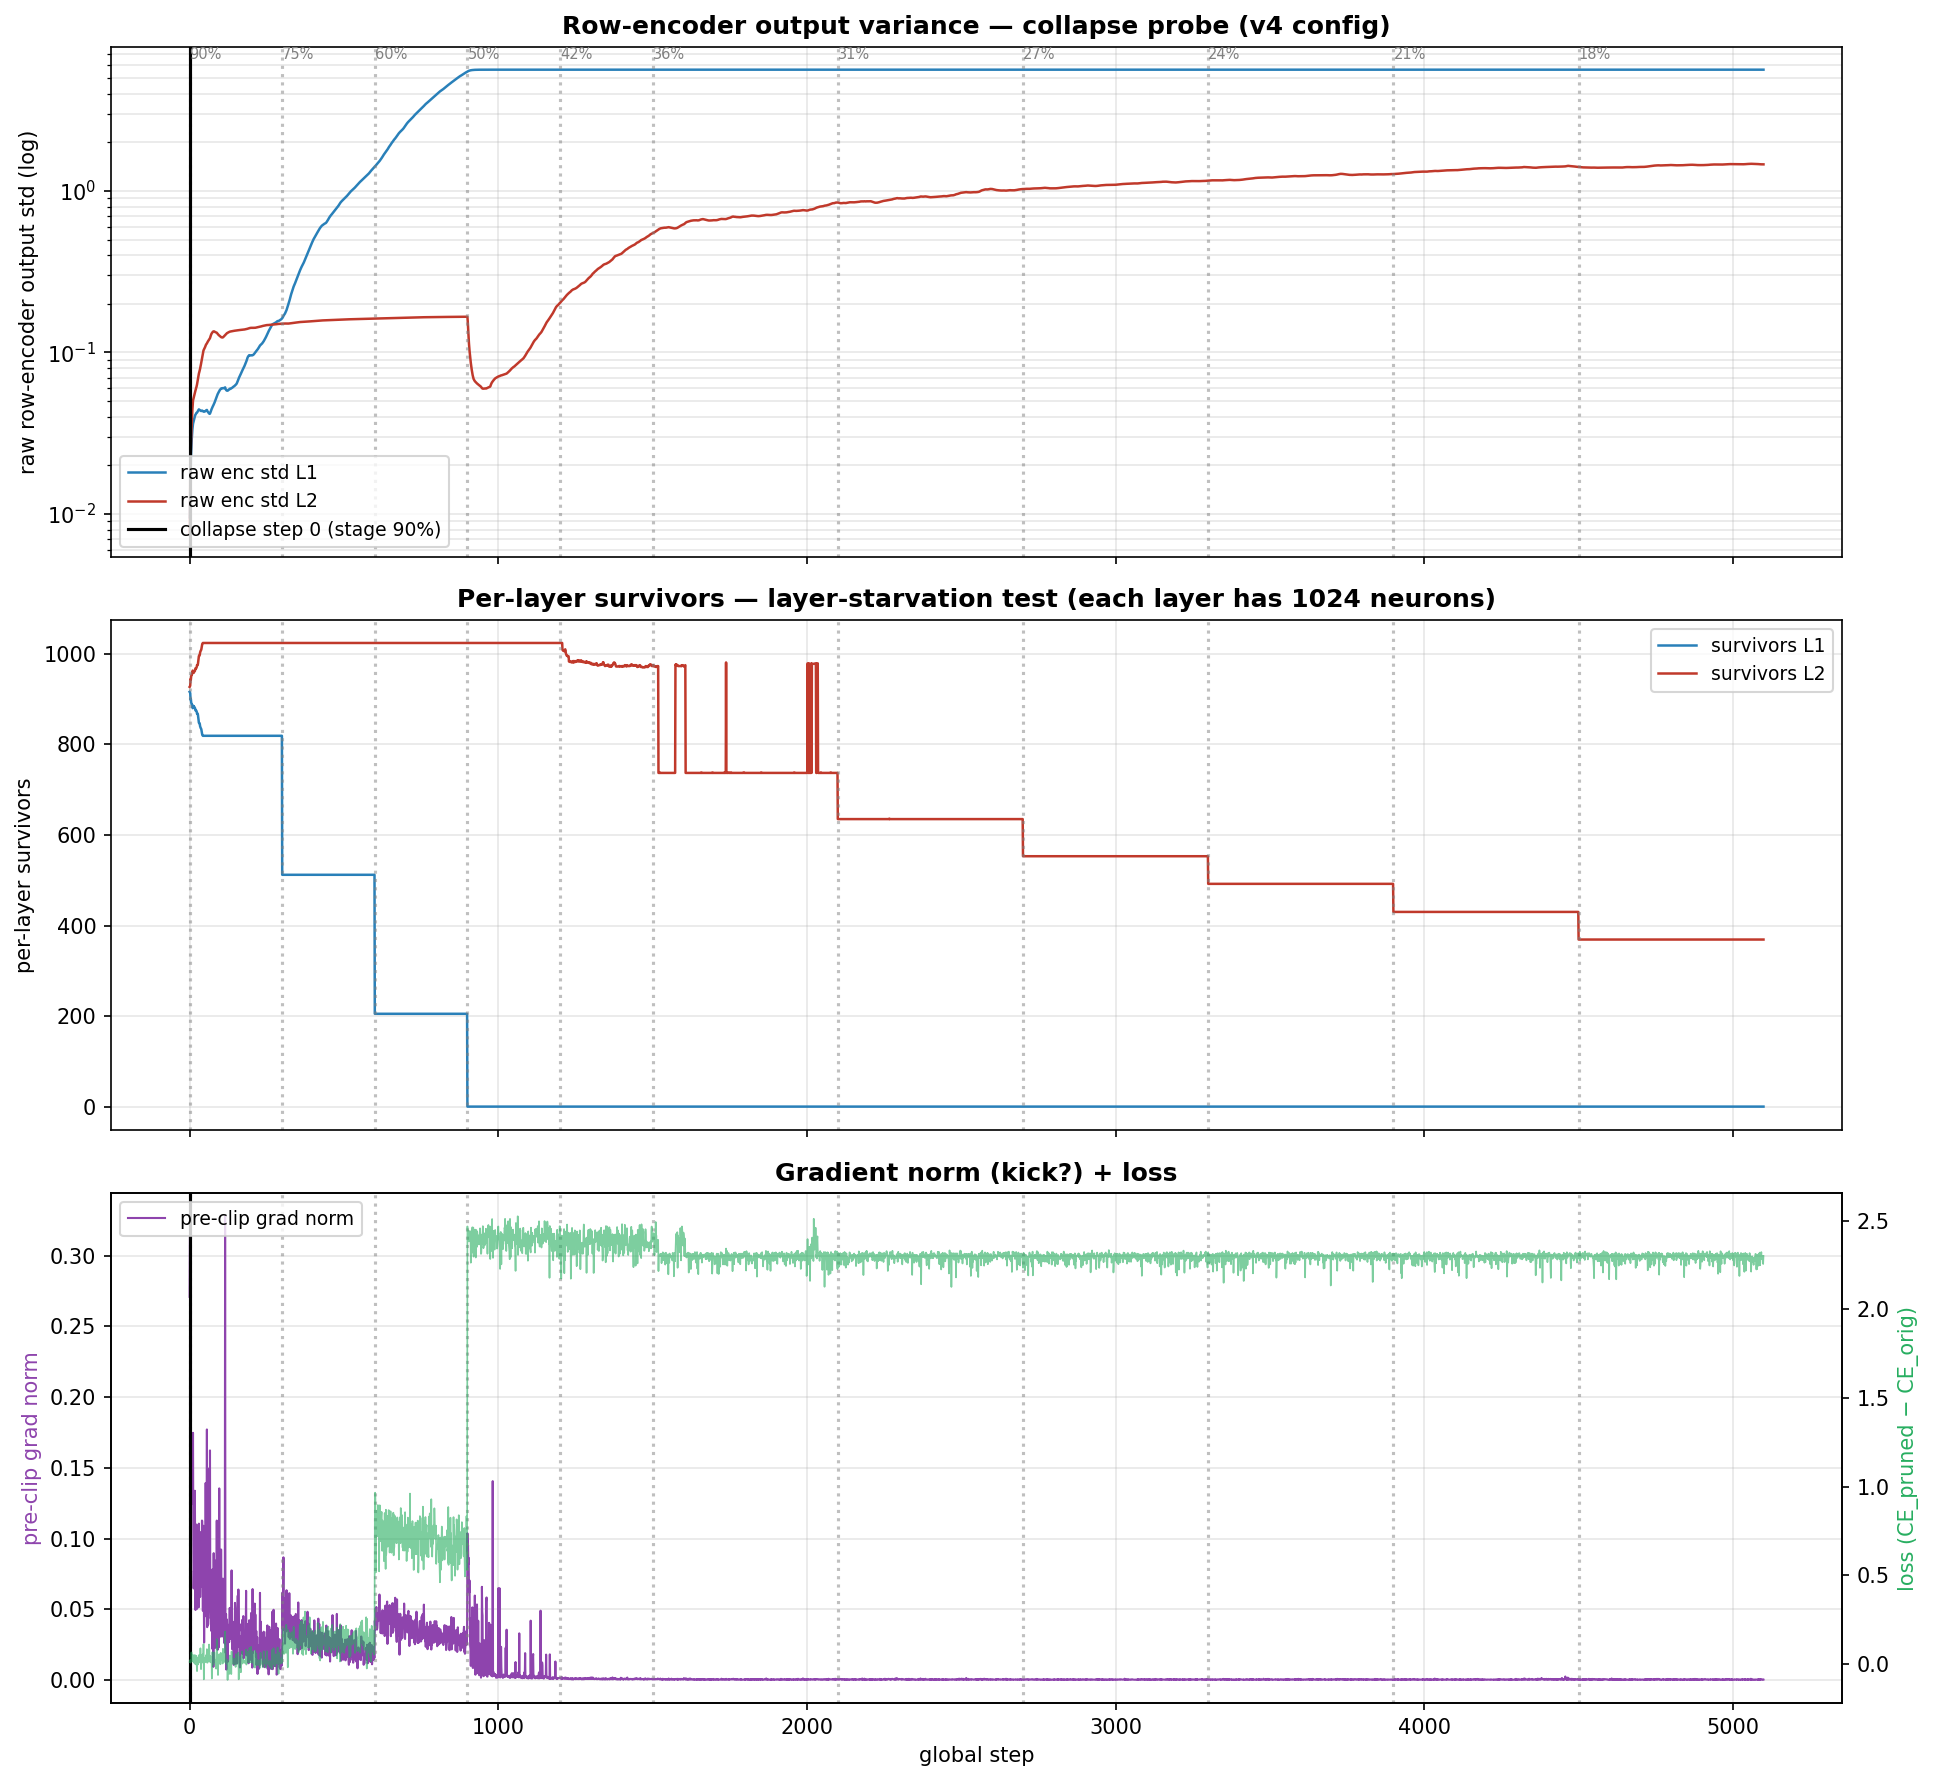
\includegraphics[width=\linewidth]{f12_starvation.png}
    \column{0.48\textwidth}
      Scores are per-layer standardised, so cross-layer allocation rides entirely on the per-layer bias $c_\ell$. Survivors:
      \[ n_\ell \approx N\big(1-\Phi(\tau - c_\ell)\big),\quad \tfrac{n_1}{n_2}\xrightarrow{\Delta\to\infty} 0 \]
      Unbounded $\Delta=c_2-c_1$ diverges $\Rightarrow$ one layer drains \textbf{819$\to$512$\to$205$\to$0} $\Rightarrow$ network severed.
      \vspace{0.4em}

      \tk{\emph{Fix:} \texttt{tanh}-bound $c_\ell\!\in\!(-1,1)\Rightarrow\Delta\!\in\!(-2,2)$. The hack we dropped was load-bearing.}
  \end{columns}
\end{frame}

\begin{frame}{Pathology \#2 --- the normalization freezes the encoder}
  \begin{columns}[T,onlytextwidth]
    \column{0.52\textwidth}
      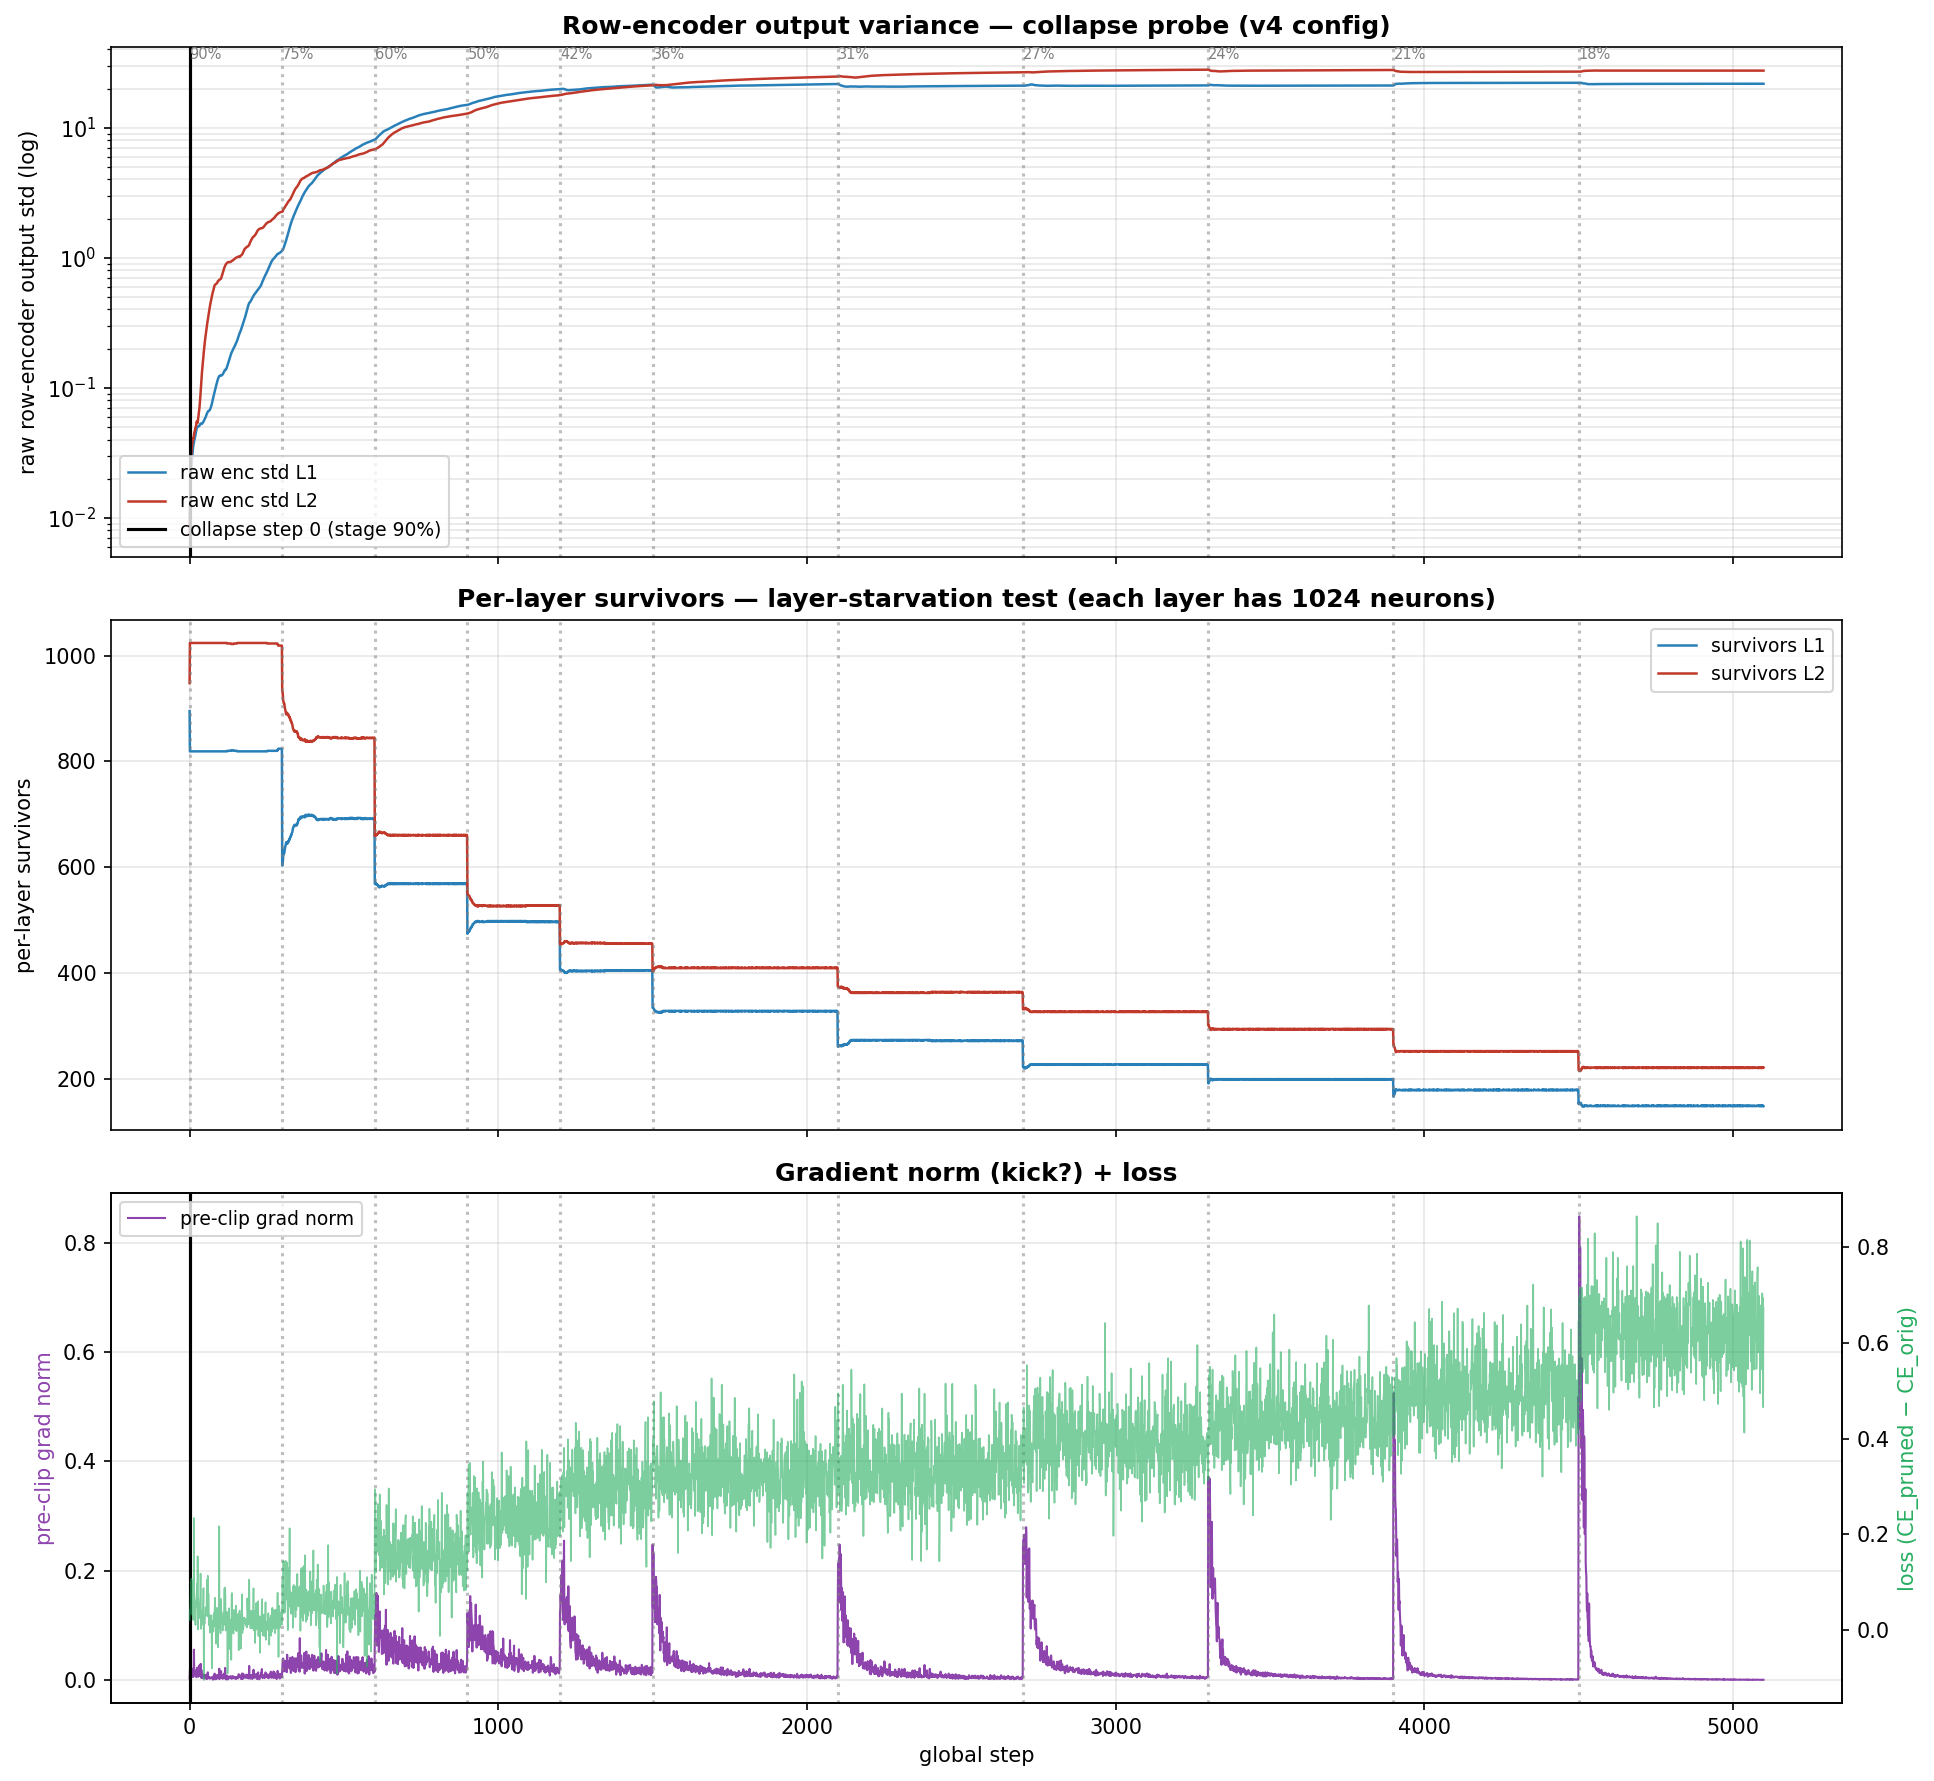
\includegraphics[width=\linewidth]{f12_center.png}
    \column{0.48\textwidth}
      Standardizing scores $y=(l-\mu)/\sigma$ is \emph{scale-invariant}:
      \[ \mathcal{L}(\alpha l)=\mathcal{L}(l)\ \Rightarrow\ \sigma \text{ is a free coordinate} \]
      So $\sigma\!\to\!\infty$, and the gradient $\partial\mathcal{L}/\partial l \propto 1/\sigma \to 0$ --- the ranking \textbf{freezes}.
      \vspace{0.4em}

      \emph{Fix:} \textbf{center-only} ($y=l-\mu$, no $/\sigma$). Not scale-invariant $\Rightarrow$ no freeze (loss runs a clean per-stage sawtooth).
      \vspace{0.3em}

      \tk{Each ``cleaner'' choice removed a guardrail $\lambda$ never needed.}
  \end{columns}
\end{frame}

\begin{frame}{Even fully de-bugged, top-K loses to $\lambda$}
  \begin{columns}[T,onlytextwidth]
    \column{0.5\textwidth}
      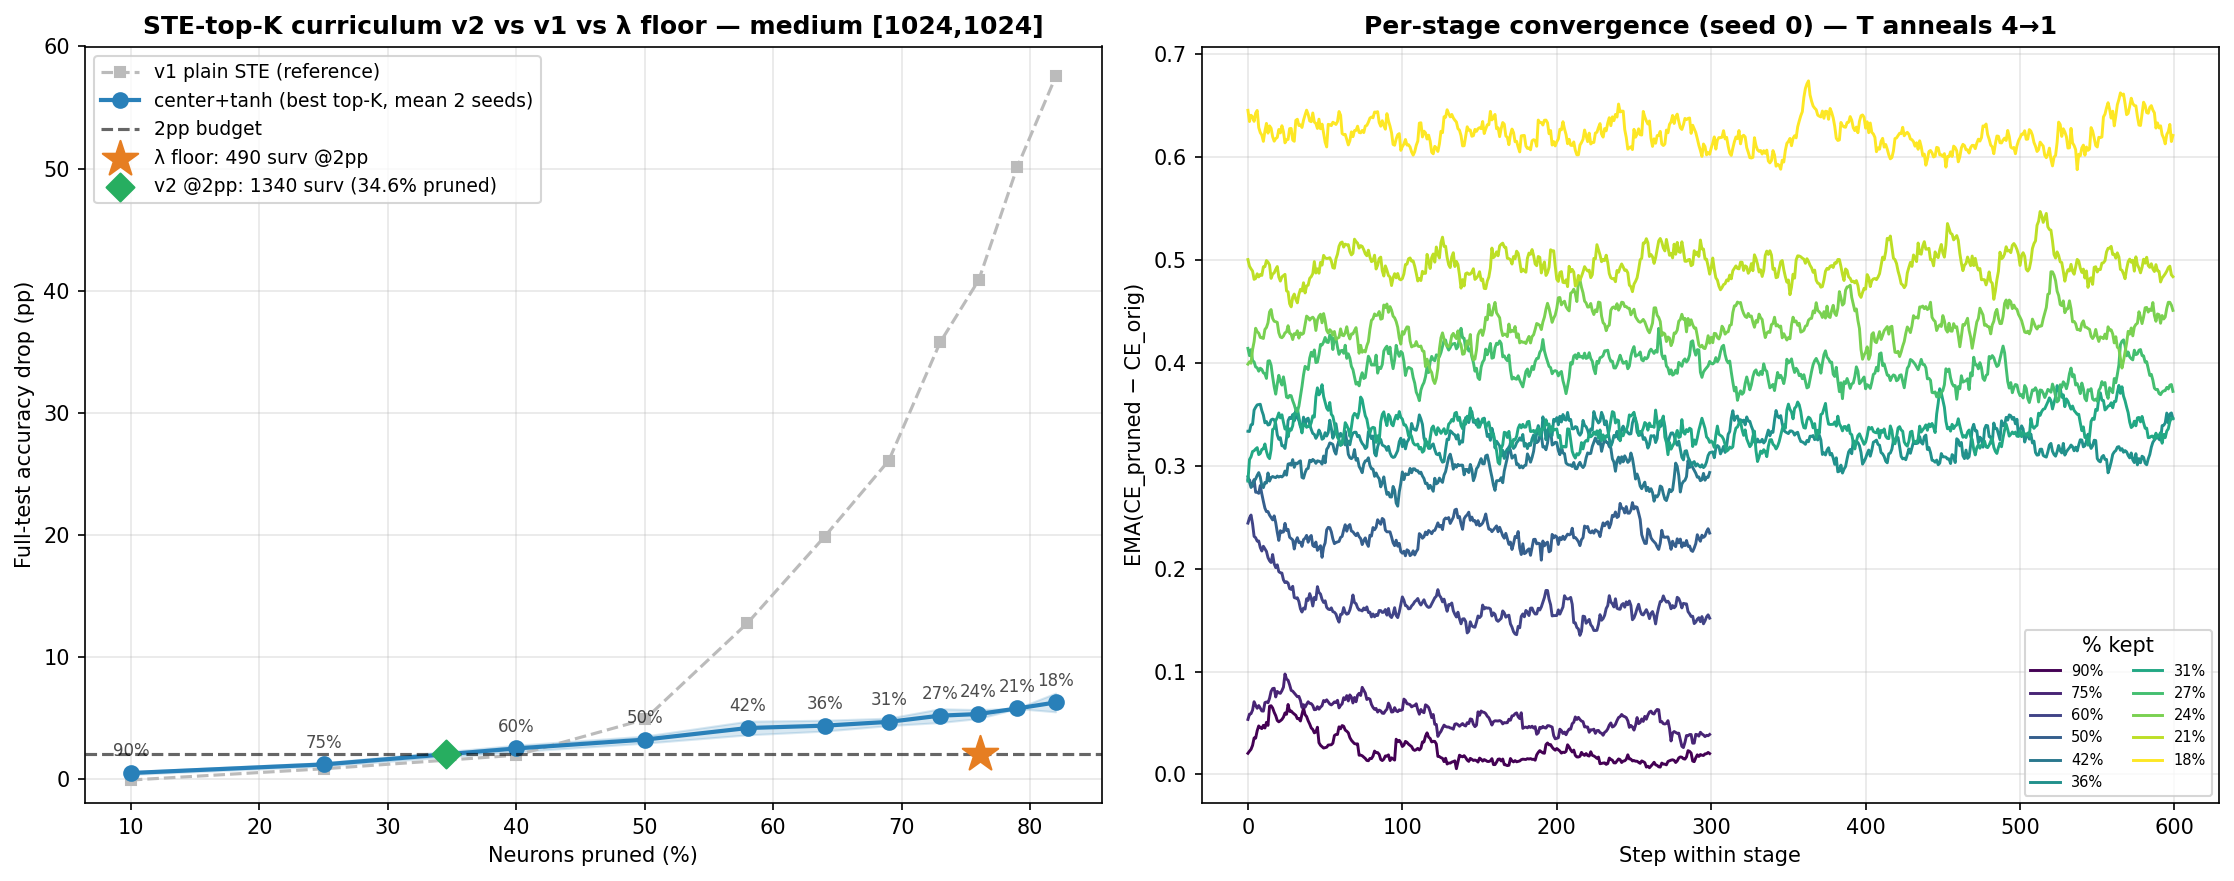
\includegraphics[width=\linewidth]{f12_final.png}
    \column{0.5\textwidth}
      \textbf{F12.} Best stable top-K (centered STE + center-only + tanh, 2 seeds, no collapse):
      \begin{center}\small
      \begin{tabular}{@{}lrr@{}}
        \toprule
        & top-K & $\lambda$ \\
        \midrule
        \% pruned @2pp & 34.6 & \textbf{76.1} \\
        drop @76\% pruned & 5.3 & \textbf{$\sim$2.0} \\
        \bottomrule
      \end{tabular}
      \end{center}
      \vspace{0.4em}
      $\sim$2.6$\times$ less pruning at iso-accuracy.
      \vspace{0.3em}

      \tk{Three pathologies; two fixed, one structural (next slide).}
  \end{columns}
\end{frame}

\begin{frame}{The structural ``why'' (Q8: the mask as instrument)}
  \begin{columns}[T,onlytextwidth]
    \column{0.5\textwidth}
      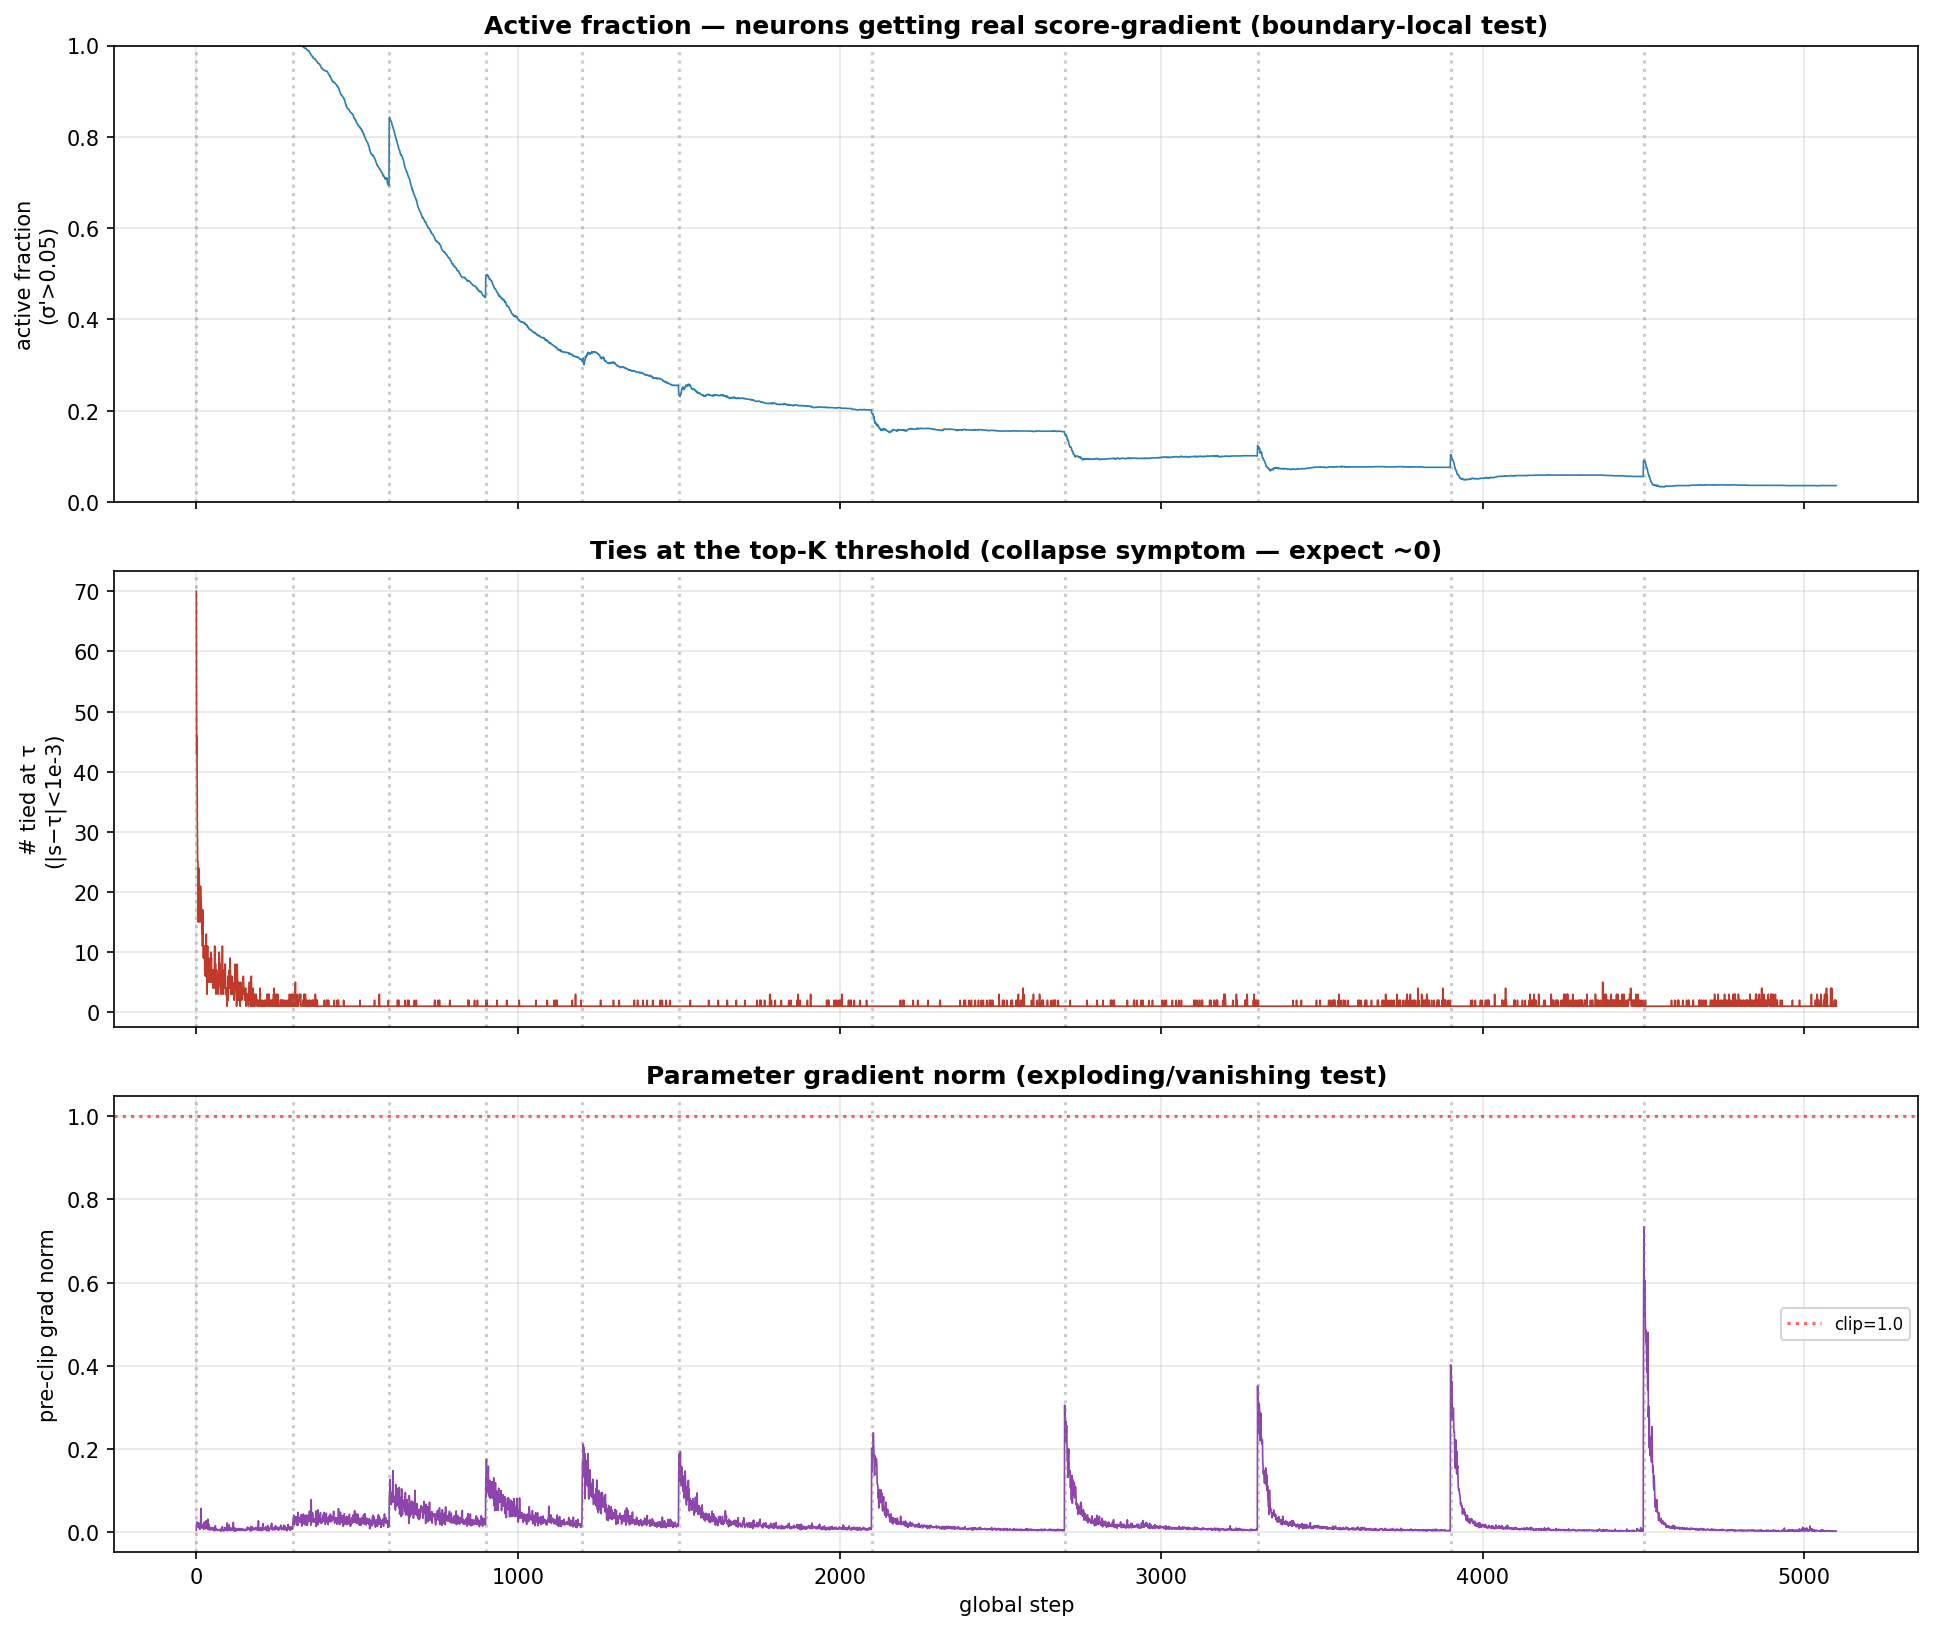
\includegraphics[width=\linewidth]{f12_proof.png}
    \column{0.5\textwidth}
      Centered-STE gradient is non-zero only near the moving threshold $\tau$:
      \[ \text{active fraction} \approx \tfrac{T}{\sigma} \]
      Measured: at the target sparsity only \textbf{$\sim$8\%} of neurons get a gradient each step --- the rest are saturated.
      \vspace{0.4em}

      \tk{Hard budget + \emph{boundary-local} gradient is a weaker subset-selection optimizer than $\lambda$'s soft \emph{global} gradient. \textbf{Sweep-free $\neq$ better.}}
  \end{columns}
\end{frame}

% ============================================================
\section{Open questions \& next steps}
% ============================================================

\begin{frame}{Open questions}
  \begin{description}
    \item[Q4] What sets prunability? \textcolor{good}{Width / redundancy distribution} --- answered.
    \item[Q9] Is there a universal minimal subnetwork? \textcolor{good}{No} --- it grows with depth; the \emph{compute} floor ($\sim$240K) is the invariant.
    \item[Q6] Is there a \emph{transferable} redundancy detector? Open --- meta-train across a distribution of nets with permutation-invariant features.
    \item[Q7] Does RL win when weights \emph{co-adapt}? Untested --- the one non-degenerate regime.
    \item[Q8] What is the pruner \emph{measuring}? Treat the (deterministic) mask as an instrument, not just a tool.
  \end{description}
\end{frame}

\begin{frame}{Next steps}
  \begin{description}
    \item[A1] \textbf{Richer input} --- feed activations / Taylor importance, not just weights. More signal at the cliff; permutation-invariant $\Rightarrow$ a shot at transfer.
    \item[B3] \textbf{Staged prune + retrain} --- iterative magnitude-style pruning with the BiLSTM scorer. The \emph{only} path past the 240K floor toward 82K.
    \item[C1] \textbf{Prune during training} --- co-adaptation makes the MDP genuinely sequential (the principled home for RL; Q7).
    \item[C3] \textbf{Alternative MDP framings} --- per-input conditional / dynamic compute, where ordering genuinely matters by construction.
  \end{description}
  \vspace{0.3em}
  \tk{Two priorities get their own slide next.}
\end{frame}

\begin{frame}{Focus 1 --- scale up to CIFAR + conv (ideas F1)}
  \begin{columns}[T,onlytextwidth]
    \column{0.55\textwidth}
      \textbf{Why.} Everything so far is MNIST MLPs. Does the story survive a harder task and a different granularity?
      \begin{itemize}
        \item Width $=$ redundancy?
        \item Architecture-invariant \emph{weight} floor?
        \item BiLSTM dominance over heuristics?
      \end{itemize}
    \column{0.45\textwidth}
      \textbf{What changes.}
      \begin{itemize}
        \item Prune \emph{channels}, not neurons.
        \item Row-encoder $\to$ per-channel filter encoder.
        \item A real compute target (FLOPs), not toy MACs.
      \end{itemize}
  \end{columns}
  \vspace{0.6em}
  \tk{This is the validation gate --- it tells us which MNIST findings are laws vs artifacts.}
\end{frame}

\begin{frame}{Focus 2 --- a self-attention pruner (ideas F2)}
  \begin{columns}[T,onlytextwidth]
    \column{0.52\textwidth}
      \textbf{The BiLSTM's limit.} A neuron sees only its own weight row $+$ \emph{one shared scalar} per layer. There is \textbf{no neuron$\leftrightarrow$neuron reasoning}.
      \vspace{0.5em}

      So it cannot directly express ``A and B are duplicates --- keep one.'' It is closer to a sophisticated magnitude scorer than a joint reasoner.
    \column{0.48\textwidth}
      \textbf{The fix: attention over neurons.}
      \begin{itemize}
        \item Each neuron attends to all others (within + across layers).
        \item Explicit pairwise redundancy.
        \item Permutation-equivariant by construction; $O(N^2)$ but $N\!\approx\!2048$ is fine.
      \end{itemize}
  \end{columns}
  \vspace{0.6em}
  \tk{This directly attacks the representer weakness --- the most principled architecture upgrade on the board.}
\end{frame}

\begin{frame}{Summary}
  \begin{itemize}
    \item \textbf{Width sets prunability; depth sets the floor.} The conserved quantity is compute ($\sim$240K MACs), not neurons.
    \item \textbf{RL is functionally non-sequential on a frozen net} --- no weight update between steps $\Rightarrow$ static subset selection $\Rightarrow$ the hypernetwork is the ceiling. Co-adaptation is the only escape.
    \item \textbf{Transfer fails for weights, works for the method.}
    \item \textbf{``Cleaner'' can be worse:} hard top-K traded a $\lambda$-sweep for three pathologies and a structural 2.6$\times$ loss --- a precise negative result.
  \end{itemize}
\end{frame}

\begin{frame}[standout]
  Thank you.\\[0.6em]
  {\normalsize\normalfont Findings: \texttt{diary/crisp-findings.md} \;|\; Code: \texttt{src/pruners/}}
\end{frame}

\end{document}
